% Chapter Template

\chapter{Chapter Roadmaps} % Main chapter title
%this should end up being roughly 10 pages


\label{Chapter4} % Change X to a consecutive number; for referencing this chapter elsewhere, use \ref{ChapterX}

%----------------------------------------------------------------------------------------
%	SECTION 1
%----------------------------------------------------------------------------------------

\section{Dissertation Paper 1: Conflict prediction using Satellite Imagery}\label{sec:ch4_paper1}
In this chapter of my prospectus, I will outline each of my three dissertation papers, including my methods, data, and plans for implementation.  My first paper, presented here, is predicated upon the results from my quantitative study, as shown in chapter \ref{sec:chapter3}.  Because of overlap between my quantitative analysis and this paper, I provide a synopsis of each major stage of my work here, and refer you to chapter \ref{sec:chapter3} for a broader discussion.

\subsection{Major Research Question}
\textit{Can satellite imagery alone be used to determine the likelihood of conflict in urban areas?}

\subsection{Proposed Data \& Methods}
\subsubsection{Data}\label{sec:ch4_paper1_data}
Our full data processing pipeline is presented in section \ref{sec:data_paper1}, and briefly summarized here. In order to test this hypothesis, we first need to determine the locations where riots and protests occurred in the past. To accomplish this, we filter events from the full ACLED database using the following criteria: \textbf{1)} include riots and protests, \textbf{2)} an event with a known specific date, \textbf{3)} and events with a neighborhood-specific geographic footprint.  This criteria generates a list of 53,307 riots and protests.  We avoid over representing any single location, by only allowing locations to appear a maximum of 500 times.  This further filters our list of potential locations to 37,728 events.  

With this filtered list, we attempt to download satellite images of these 37,728 riots or protests.  Our strategy to download images is to search for satellite images from 24-48 hours prior to the riot or protest.  Also, we only consider images that contain 50\% or less cloud cover.  Under these constraints, we download 19,902 satellite images.  We will use these satellite images to construct our data set.

From each satellite image, we clip a 1 \textit{$\ km^{2}$} box centered on the latitude and longitude of the riot or protest.  We label these clipped images as "riot" in our data set.  The next task is to generate up to 10 null clips, each of which is a 1 \textit{$\ km^{2}$} box.  For each satellite image we use the following criteria: \textbf{1)} null clips must be a minimum of 10 km away from the riot, \textbf{2)} null clips must be from urban regions of the satellite image, \textbf{3)} null clips are spaced far enough apart, so that none of the null clip 1 \textit{$\ km^{2}$} boxes overlap.  We label these clipped images as "nulls" in our data set.

This generates a data set that consists of 1 \textit{$\ km^{2}$} boxes, that are labeled either "riot" or "null".  Specifically, the data set contains 18,631 "riot" images, and 186,310 "null" images.  In total, the data set has 204,941 images that we can use in training.


\subsubsection{Methods}
In order to determine the likelihood of a protest or riot, we train a ResNet18 convolutional neural network.  Starting with a pre-trained ResNet18, we can train the network to predict if clipped images are from riots/protests or from null locations.  Additionally, we explore the explainability of these clipped images using Score-CAM.  We also subset our data to explore any region or cultural patterns that might emerge in our analysis.   Our full implementation is discussed in section \ref{sec:methods_paper1}.


\subsection{Possible Challenges/Barriers}
During initial investigation into this topic, there were a few limitations that we encountered.  Some of these, such as explainabiliy limitations, have lead to future research areas.  I hope to explore many of these topics as a part of my broader dissertation.

\subsubsection{Satellite Information} \label{sec:limits.satinfo}
The satellite imagery we incorporated into this study had a number of notable limitations. First, while a satellite scene might contain 50\% or less cloud cover (see figure \ref{fig:cloudy_brazil}), the clipped images might be completely covered in clouds (see, for example, figure \ref{fig:cloudy_clips}).  Further, in some cases the conflict event selected may be at the edge of a scene, with no valid scene available to fill in null information, resulting in a partially clipped image (see figure \ref{fig:poorclips}).  Additionally, some of the clips contain interference or distortion, such as the clip at the bottom of figure \ref{fig:poorclips}.

Inter-related with these challenges, in many scenes we were unable to identify enough geographic locations to support the creation of 10 null cases. For example, in figure \ref{fig:coastline_clip} we can see that the riot location in consideration does not have any null location possibilities due to the riot's proximity to the coast, and the concomitant lack of proximate urban areas eligible for building null (no-protest) cases. There are similar limitations that cause the distribution of clipped images in figure \ref{fig:null_hist}.
\begin{figure}
    \centering
    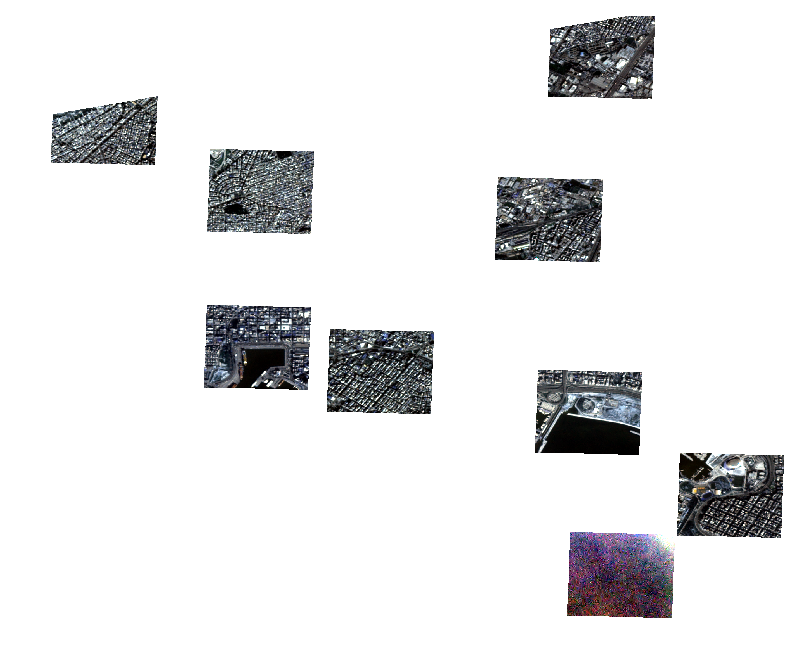
\includegraphics[width=0.5\linewidth]{poor_clips.png}
    \caption{9 of the null riot clipped images from Athens, Greece. Imagery \textcopyright Planet Labs PBC 2023. All rights reserved.}
    \label{fig:poorclips}
\end{figure}

\begin{figure}
    \centering
    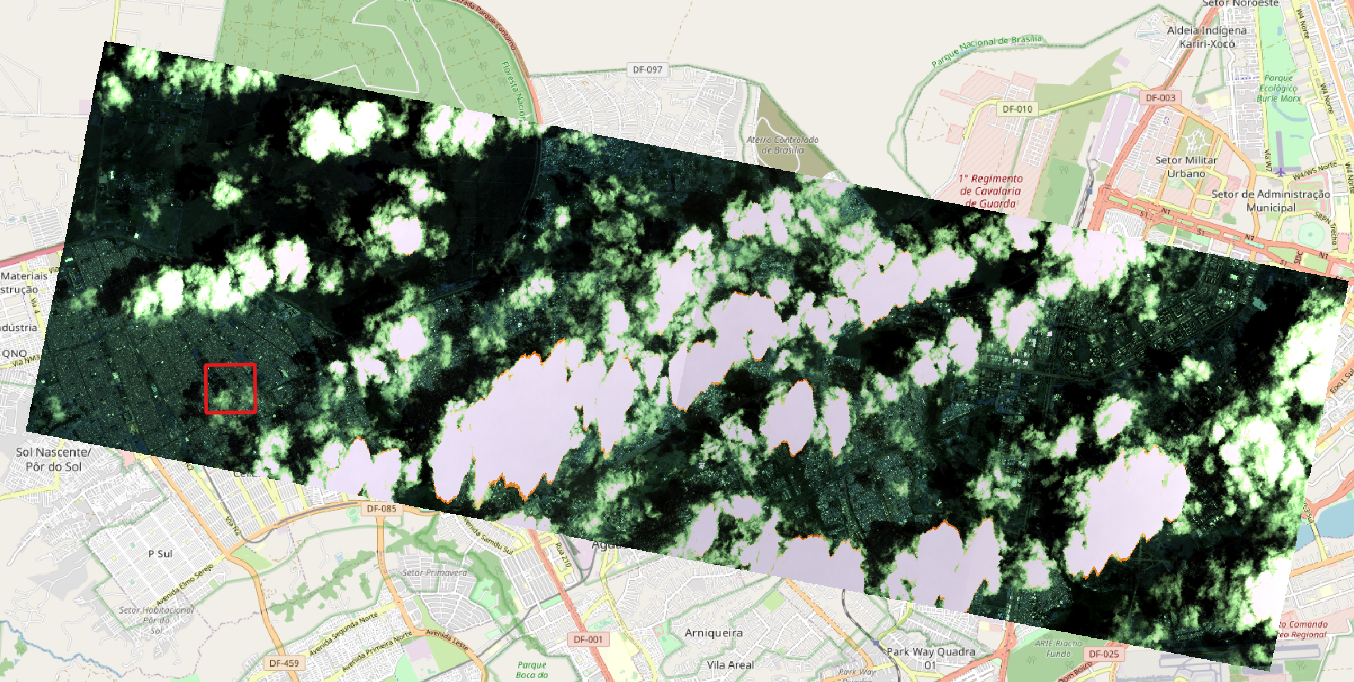
\includegraphics[width=0.75\linewidth]{cloudy_brazil.png}
    \caption{Satellite image of Brazil collected on 1 November 2018.  This image contains less than 50\% cloud cover for the full satellite scene.  The riot location indicated in the red square has minimal cloud cover, but other locations in the scene will be impacted by the cloud cover as seen in figure \ref{fig:cloudy_clips}. Imagery \textcopyright Planet Labs PBC 2023. All rights reserved.}
    \label{fig:cloudy_brazil}
\end{figure}

\begin{figure}
    \centering
    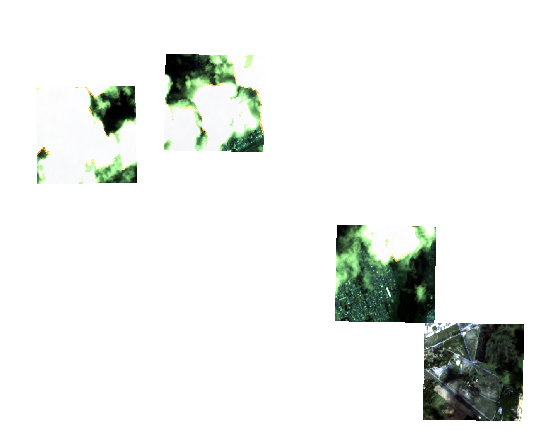
\includegraphics[width=0.5\linewidth]{cloudy_clips.png}
    \caption{Clips from a satellite image of Bazil collected on 1 November 2018.  While the full image contains less than 50\% cloud cover, many of the clips are partially or completely obscured. Imagery \textcopyright Planet Labs PBC 2023. All rights reserved.}
    \label{fig:cloudy_clips}
\end{figure}

\begin{figure}
    \centering
    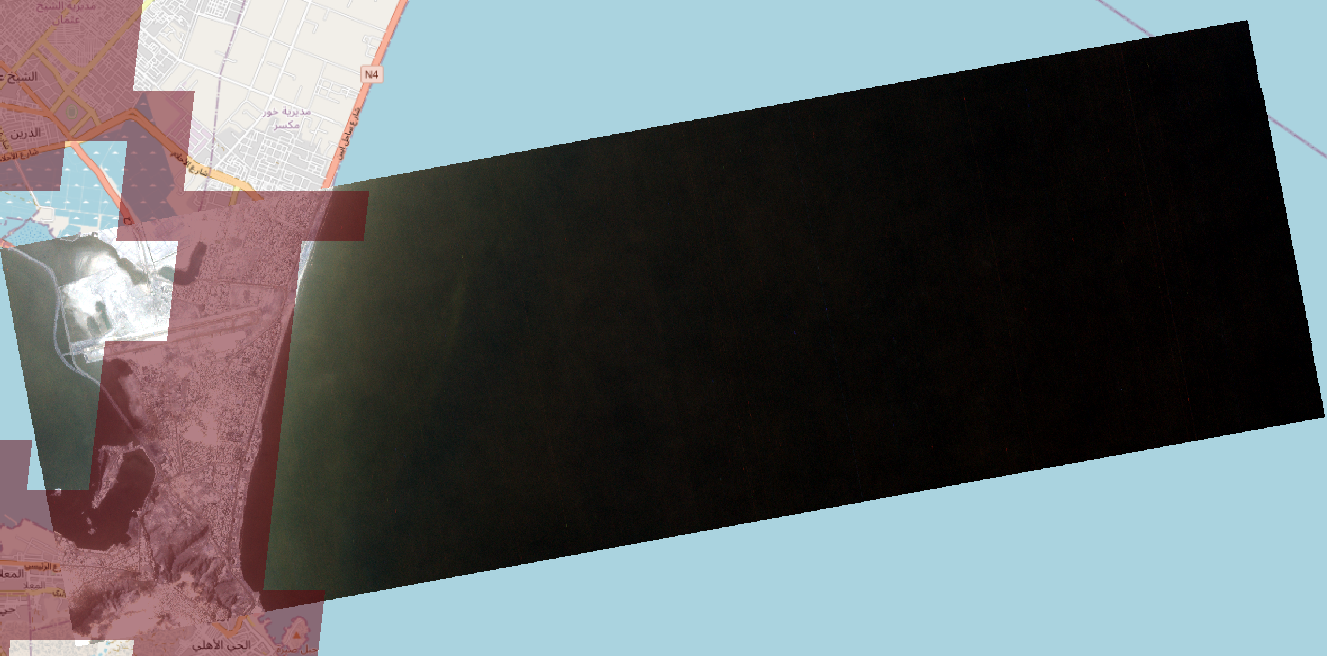
\includegraphics[width=0.75\linewidth]{coastline_clip.png}
    \caption{Satellite Image from Yemen collected on 14 September 2020.  The urban areas are shown in red.  Most of this image is not usable because of the lack of urban areas. Imagery \textcopyright Planet Labs PBC 2023. All rights reserved.}
    \label{fig:coastline_clip}
\end{figure}

Another limitation is in our definition of where conflict events occurred, as the definition of a ``neighborhood'' is inherently imprecise.  We used OpenStreetMaps \citep{OpenStreetMap2024} to visually compare the size of our ten most repeated locations \ref{tab:occurrence}.  We were able to confirm that the sizes of neighborhoods were inconsistent, but rarely of a size greater than our 10 square kilometer exclusionary zone (see figure \ref{fig:athens_nullclips}). 

To overcome this limitation, a future research direction might include ways to filter out clipped images with clouds or distortion.  Additionally if we only exclude clipped images within 1 km of the edge of the satellite scene, we could avoid images with only partial satellite information.  The neighborhood limitation is more difficult to account for, but we might group locations by their average neighborhood size and train the groups individually in an attempt to train our network to learn patterns that account for neighborhood size differences.

\begin{figure}
    \centering
    \begin{subfigure}[b]{0.45\linewidth}
        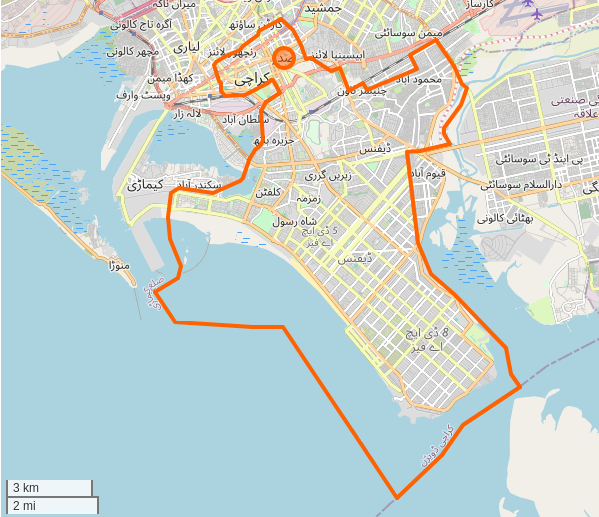
\includegraphics[width=\linewidth]{Karachi_Saddar.png}
        \caption{Karachi - Saddar }
    \end{subfigure}
    \quad 
    \begin{subfigure}[b]{0.45\linewidth}
        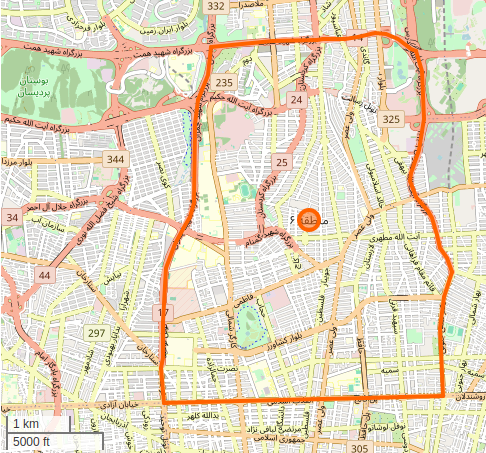
\includegraphics[width=\linewidth]{Tehran_District6.png}
        \caption{Tehran - District 6}
    \end{subfigure}
    \begin{subfigure}[b]{0.45\linewidth}
        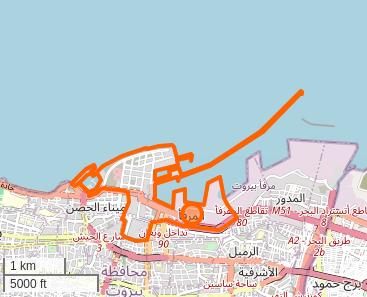
\includegraphics[width=\linewidth]{Beriut_Port.png}
        \caption{Beriut - Port}
    \end{subfigure}
    \quad 
    \begin{subfigure}[b]{0.45\linewidth}
        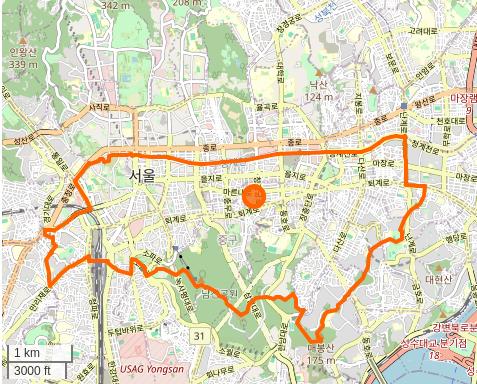
\includegraphics[width=\linewidth]{Seoul_Jung.png}
        \caption{Seoul - Jung}
    \end{subfigure}
    \caption{Four example neighborhoods from the top ten repeated locations.  The scale of the image is given in the lower left corner of each image. 
 The size of the neighborhoods is not consistent across the globe, but based of the labels in OpenStreetMap\citep{OpenStreetMap2024}, our methodology of excluding 10-km around the neighborhood will force our null cases to generate from locations outside the given neighborhood.}
 \label{fig:neighborhoods}
\end{figure}

\subsubsection{Explainability}\label{sec:explainability}
Currently, the majority of explainability techniques in the literature are focused on datasets consisting of object-centric images.  For example, two common data sets CIFAR-10 and CIFAR-100 \citep{cifar10_100} are used in many computer vision tasks and competitions, but those data sets only have objects centered in the middle of the picture, taking up most of the image space.  This differs significantly from our satellite imagery.  Our images contain all of the spatial information within a square kilometer in a city.  As opposed to an image of a cat or dog, our images have multiple buildings, cars, streets, parks, etc.  So while current explainability techniques can highlight portions of our image that lead to classification which are easily human interpretable, it is challenging for us to determine what in the image is being highlighted.  The example we discussed previously, sports stadiums, are identified in Score-CAM and easily identified visually in the satellite image.  There were other patterns that emerged in our Score-CAM analysis; however it is very difficult to describe many of the features Score-CAM identifies with easily identifiable semantic definitions. While we were able to identify a few other patterns, such as transitions from one zone to another zone (residential to commercial as an example), we are not confident in interpreting what these different types of zones are at this time.  The field of explainability, as it relates to satellite images, has very little published in literature and remains a strong avenue for future inquiry.

To overcome this limitation, a future research direction is outlined in section \ref{sec:paper_two}.  We intend to explore better understanding objects and spatial features identified by Score-CAM, through the use of points of interest identified in open source databases such as Overture Maps \citep{OvertureMapsFoundation2023}.  This would require segmenting the results of Score-CAM and comparing the objects indicated in Overture, to determine if there are patterns that arise indicating a riot or non-riot.  

\subsubsection{Additional Limitations}
There are a number of additional limitations of the presented work. 
 First, our data is focused on spatial information, not temporal, and thus we do not generate predictions of \textit{when} a riot will occur, only the likely urban locations.  Leveraging changes in images over time could help us overcome this challenge, but will necessitate new modeling strategies beyond those presented in this piece. Second, we have selected a ResNet18 as our base model, which could limit our model performance if alternative architectures are better performing. 

Third, the ACLED database used to construct our imagery data set is drawn primarily from news sources \citep{acled_codebook_2023}.  These comes with some inherent challenges and limitations.  If riots and protests are occurring in regions that traditional news sources are not reporting about, the events are not likely to populate the ACLED database.  Further, the nature of civil unrest is sometimes difficult to delineate with clear definitions, and different news organizations may cover a protest in conflicting ways - for example, a protest that is met with armed government resistance \citep{acled_codebook_2023}.  These challenges are not likely to be overcome in the near term, but are notable as they may impact the results presented in this study.

To overcome this limitation, a future research direction might include downloading new images from weeks or months before the riot, as well as images from after the riot date.  This would provide temporal differences for us to train our model to learn to differentiate.  We could do this with a ResNet, or attempt to train with alternate architectures.  To account for biases that might be present in the ACLED database, we might investigate alternate events within ALCED, or different databases.  


%----------------------------------------------------------------------------------------
%	SECTION 2
%----------------------------------------------------------------------------------------

\section{Dissertation Paper 2: Explainability in Satellite Imagery} \label{sec:paper_two}
While initial results from my first dissertation paper indicate that satellite imagery can be used to predict - with up to 97\% accuracy - where riots and protests are likely to occur in an urban area, it provides no insights into \textit{what features in the image are important}.  This is a critical step, as for policymakers to learn from or trust this model, we must understand the key on-the-ground factors that the model is leveraging. Thus, while my first chapter focused on the estimation of the location of a conflict event, in this chapter I will focus on explaining the features that were actually used.  


\subsection{Major Research Question}
\textit{Can we semantically describe the features within a satellite image that are consequential to the classification of urban conflict?}

\subsection{Data}
The core satellite imagery data used for this analysis will be the same dataset described in section \ref{sec:ch4_paper1_data}. This dataset provides over 2,178 images, which are each labeled as either a location at which protests or riots occurred, or an area drawn from the same urban environment at which no event occurred (see figure \ref{fig:athens_nullclips}).  Each of these images is a 1 \textit{$\ km^{2}$} box centered around a known riot/protest, or a non-riot location from the same satellite image as the riot clip. As a part of the quantitative analysis presented in Chapter \ref{sec:chapter3}, this data has already been acquired and processed. 

In addition to satellite imagery, this paper's activities will require a method through which the features that are identified as important on the ground are semantically labeled.  For example, a series of pixels that appears to represent a football stadium may be highlighted; in order to programmatically identify that location as a football stadium, we require a broad source of place names that we can correlate with the highlighted location. To accommodate this, we will leverage data sources from open source repositories, including SpaceNet\citep{SpaceNet}, DeepGlobe\citep{DeepGlobe2018}, xView\citep{xView}), Open Street Map \citep{OpenStreetMap2024}, and/or Overture Maps \citep{OvertureMapsFoundation2023}. All of these are open source and freely available, but at this time it is unknown which of these - or which combination of these - will be best suited for our purposes.

\subsection{Methods}
Our core aim is, given an image of a location and a deep learning model designed to estimate if conflict is likely to occur at that location or not, provide a human-understandable, semantic description of why the model made a given decision.  An output of this approach may be a sentence similar to one of these examples:\\
``It is likely that a riot will occur in this area, as it is proximate to numerous pubs and large public gathering spaces, in an area with a historic proclivity for riots.''\\
``It is unlikely that a riot will occur in this area, as there is a lack of large physical spaces in which crowds could aggregate.''\\
``We estimate, with 85\% confidence, that a riot is likely to occur in this area.  The key indicators included the presence of government properties and large fields in which aggregations can occur.''

In order to accomplish this, we propose a multiple-step process, in which:
\begin{enumerate} [itemsep=-1ex]
    \item We implement a modified Score-CAM (SAT-Cam) to capture the pixels which were important to the model's decision function.
    \item We threshold and then identify place names near the most important areas.
    \item We validate based on consensus between data sources and human labeled observations.
\end{enumerate}

\subsubsection{Step 1. Modified Score-CAM}
To date, explainability techniques in computer vision have predominantly emerged from traditional application - such as seeking to understand why an image taken from a cellphone is a cat or dog.  As noted in the introduction to this prospectus, this has resulted in a number of limitations when it comes to applications for satellite imagery-based analyses.  Critical themes include: \textbf{1.} Many current explainability techniques focus on images with a single object in the scene, satellite imagery by nature has many objects present in the same scene.  \textbf{2.} Satellite imagery will have less variance in pixel values when compared to other images used in computer vision tasks, which will make understanding which spatial features are important in classification challenging to decipher.  \textbf{3.} Semantic definitions are unclear in many satellite images, which will require us to use third-party data sources to distinguish features identified in explainability techniques.   

% \begin{enumerate} 
% \item \textbf{Multi-target limits} Many current explainability techniques in litureature focus on single objects \\
% \item Satellite imagery have significantly less variance in pixel values than other classes of data.\\
% \item Semantic definitions are unclear in many cases, forcing a reliance on third-party data sources.
% \end{enumerate}

In order to overcome these limits, we propose a modified implementation of Score-CAM.  Score CAM is a class activation map explainability method that utilizes weights as opposed to gradient in the model.  This method has demonstrated the ability to handle multi-target images better than other CAM methods \citep{wang2020score}.  It is formally defined as: 

\begin{equation}
\centering
L^{c}_{Score-CAM} = ReLU (\sum_{k} \alpha^{c}_{k} A^{k}_{l})  
\label{score-cam_equation}
\end{equation}
$\ A^{k}_{l} $ is the activation map for $\ k^{th} $ channel of layer \textit{l}, and $\ \alpha^{c}_{k} $ is the weight associated with the $\ k^{th} $ neuron. Where $\ \alpha^{c}_{k} = C(A^{k}_{l}) $ for convolutional layer \textit{l} and a class of interest \textit{c}. And $\ C(A^{k}_{l}) $ is the channel-wise increase of confidence introduced with Score-CAM.  \citep{wang2020score}.  

In order to overcome issues associated with multi-target limits and variance, we propose two changes to Score-CAM.  This revised algorithm, which we label "SAT-CAM", takes the following functional form:

\begin{equation}
L^{c}_{\text{SAT-CAM}} = \text{ReLU}\left(\sum_k \left\{
\begin{array}{cl}
\alpha_c^k A_k^l & \text{if } \alpha_c^k A_k^l > \epsilon \\
0 & \text{otherwise}
\end{array}
\right.\right)
\label{sat-cam_equation}
\end{equation}

Where $\ L^{c}_{SAT-CAM} $ is the output of SAT-CAM, that thresholds the Score-CAM evaluation $\ ReLU (\sum_{k} \alpha^{c}_{k} A^{k}_{l})$ by $\ \epsilon$.  In effect, this removes pixels below the threshold $\ \epsilon$ for consideration.

The output of SAT-Cam is a heat map matrix of the activation layer $\ A^{k}_{l} $ in which highlighted pixels contributed to the decision function.  Building on Score-CAM, $\ A^{k}_{l} $ is the last convolutional layer before the first fully connected layer.  This is passed into the next stage of the process, in which we seek to use ancillary geographic databases to semantically label the regions of the image that are identified as important.

\subsubsection{Step 2. Threshold \& Identifying Place-Names}

Using the output generated from SAT-CAM in equation \ref{sat-cam_equation}, we will apply a segmentation algorithm \citep{kirillov2023segment}, and then select the top 1 to 3 segments in terms of their absolute average value of importance.  Once selected, we will test three different approaches to semantic interpretation (two stand-alone approaches, and one integrated).  These are:
\begin{enumerate}
\item Clipping the underlying satellite imagery and passing it into an existing classification model. 
\item Identifying the place-names that are proximate to important areas from ancillary geospatial databases, and integrating them into a human-readable form. 
\item Providing both types of information into a large language model (LLM) to create a human-interpretable semantic description. 
\end{enumerate}


In the first approach, we seek to have a separate computer vision model label the isolated regions with their predominant structural characteristics.  For example, there are a number of challenges, SpaceNet Challenge \citep{SpaceNet}, DeepGlobe Challenge \citep{DeepGlobe2018}, and xView Detection Challenge \citep{xView}, that identify and label objects in satellite imagery.  This will leverage existing models, such as SpaceNet to decipher what objects are in the imagery.  If we apply these models to our regions of interest, we can generate a list of objects that appear frequently in our data.  By analyzing the results we might be able to determine what objects or spatial characteristics and features are critical in classification.

In the second approach, we will leverage data from sources such as Overture Maps \citep{OvertureMapsFoundation2023} and Open Street Map \citep{OpenStreetMap2024} to identify important place names proximate to the important features in geographic space.  First this will require construction of segments that contain the regions of interest identified in SAT-CAM.  These segments will have to be properly geo-referenced, so we only capture points of interest relevant to classification.  Using these segments as limiting constraints, we will then generate a list of the points on interest from Overture, as an example.  

These databases contain many types of information that might prove useful in explaining classification.  Overture Maps Foundation \citep{OvertureMapsFoundation2023}, for example, contains over 59 million locations.  Each location in the Overture map data contains not only location information (latitude and longitude), but also some class information, such as "residential", "commercial", or "education."  There are many land use classes as well, with examples such as "agriculture", "airport", "park", "recreation", "religious", and many more.  

This approach generates a list of location names, classes, and land uses for every segment identified by SAT-CAM.  Additionally, we have the classification of the overall image from the ResNet (riot or non-riot), the output of the final fully connected layer, and the accuracy of the classification (True Positive, False Negative, etc).  There is the potential to then leverage a LLM (Large Language Model) to help describe what is important in explaining classification.  A diagram displaying the data generation that will be used as input into the LLM is shown in figure \ref{fig:paper2_flowchart}.  At this point, all of the inputs would be text, and a trained LLM may be able to provide useful semantic descriptions given both the satellite-derived and gazetteer-based inputs.


\begin{figure}
    \centering
    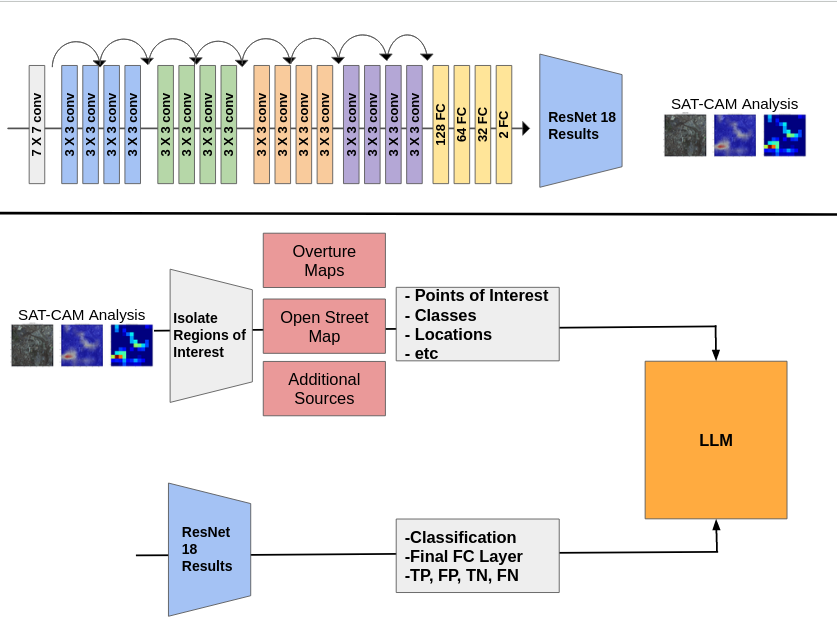
\includegraphics[width=0.75\linewidth]{Figures/paper2_data_flowchart.png}
    \caption{Flow chart detailing inputs into LLM.  We will use the outputs of our ResNet18 and SAT-CAM analysis to feed text into an LLM. }
    \label{fig:paper2_flowchart}
\end{figure}


A third approach, we will use a hybrid between the first two, in which a LLM will receive an input a prompt that contains all of the text input highlighted in the second approach (see figure \ref{fig:paper2_flowchart}) with the classification model utilized in the first approach.  This approach is more complicated, but leverages both the visual classification models that already exist and additional information about the segmented regions available in open source database.  

\subsubsection{Step 3. Validation}

There are two potential courses of action for validation of SAT-CAM, human labeling and consensus of databases.  The first viable option is to simply have individuals label by hand the relevant regions of interest and compare the human labels with the SAT-CAM labels.  This would be an relatively straightforward method when there is a single region of interest and a single human generated label.  However, as the number of regions of interest or the size of the regions increase, there will be an associated increase in the amount of data humans are required to label.  This increase spatial area has an accompanying increase in challenge and ambiguity.  For example, if half of a clipped image is categorized as important by SAT-CAM, half a square kilometer of an urban area must be labeled by a human.  Human labeling might prove easier to implement for smaller SAT-CAM results, and difficult to implement for large SAT-CAM results.

The second viable option for validation could be consensus.  The results of the SAT-CAM analysis require access to databases with labeled locations.  Once the methodology and data pipelines are established to evaluate a clipped image with SAT-CAM and generate a list of points of interest that exist within the segmented satellite data, the process can be replicated with different open source data bases.  If the list of locations for Overture Maps, Open Street Map, and potentially others, all agree, then the list is most likely an accurate representation of the spatial features important for classification.  



\subsection{Possible Challenges/Barriers}
There are a number of possible challenges to the successful execution of this work.  First and foremost is a lack of relevant past literature on which to build.  The majority of prior work in literature pertaining to computer vision uses data sets and examples that are object-centric.  Much of the prior work uses standard data sets such as CIFAR-10 and CIFAR-100, which consist exclusively of photographic images, with the object centered in frame.  Satellite imagery is very different in practice.  The dataset under examination in this study comprises satellite imagery, distinct from conventional photographs, encompassing spatial regions of interest that may appear at any location within the image frame, rather than being centrally positioned. This characteristic marks a significant departure from the datasets predominantly utilized in existing literature. 

Another potential challenge is that the Score-CAM results will contain both contiguous and non-contiguous results.  If all of the regions of interest are contiguous (as in figure \ref{fig:contiguous_ScoreCAM}), the association of the single region as the single entity that is important to classification is straight forward.  However, there are other Score-CAM results that are not contiguous (see figure \ref{fig:noncontiguous_ScoreCAM}), and it is unclear if these regions should be evaluated individually or collectively.  

Determining how to treat these non-contiguous areas as a non-overlapping polygons in the explainability research is similar to the object based image analysis (OBIA) challenge of analyzing images and objects at the appropriate resolution to avoid the "salt and pepper effect" \citep{blaschke2010object}.  So while there is similar work with satellite imagery, in fields such as OBIA, there is little work exploring the potential obstacles associated with explainability.  The non-contiguous nature of important features in satellite imagery could cause a number of challenges, opening a number of areas for inquiry.  Questions include: 
Is the classification determined by the sum of all weights or regions, or the maximum weight of a single region?
What role do interaction effects of non-contiguous regions play in classification?
Does the spatial distance between non-contiguous regions impact the classification of the image?
These challenges are specific to the use of explainability techniques in satellite images.

% \begin{figure}
%     \centering
%     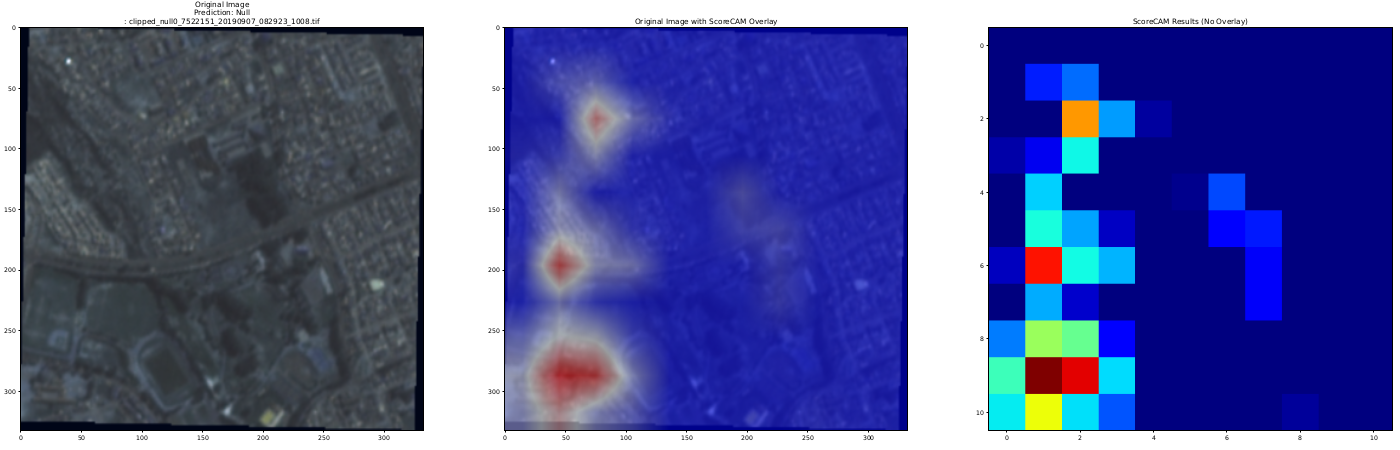
\includegraphics[width=1\linewidth]{stadium_scorecam2.png}
%     \caption{Example clipped image on the left.  The clipped image, a one kilometer box around a non riot location.  The Score-CAM overlayed on top of the image is shown in the middle.  The Score-CAM visual is displayed on the right }
%     \label{fig:score_cam_stadium2_ch4}
% \end{figure}

\begin{figure}
    \centering
    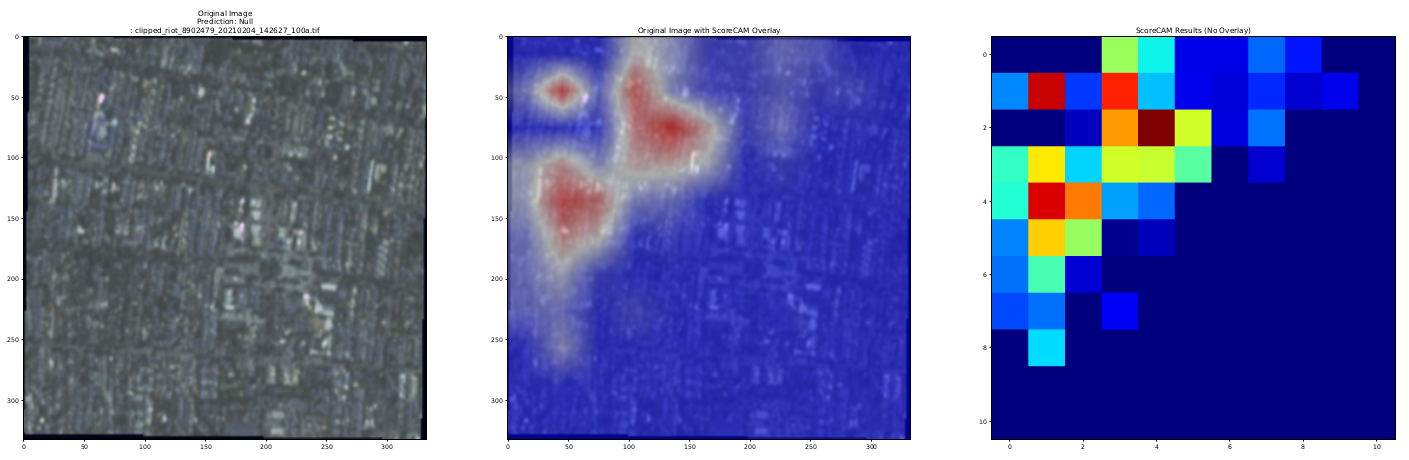
\includegraphics[width=0.75\linewidth]{contiguous_results.png}
    \caption{Score-CAM results displayed on the right of this figure represent a single contiguous region, regardless of the threshold set for consideration into a region of interest.}
    \label{fig:contiguous_ScoreCAM}
\end{figure}

\begin{figure}
    \centering
    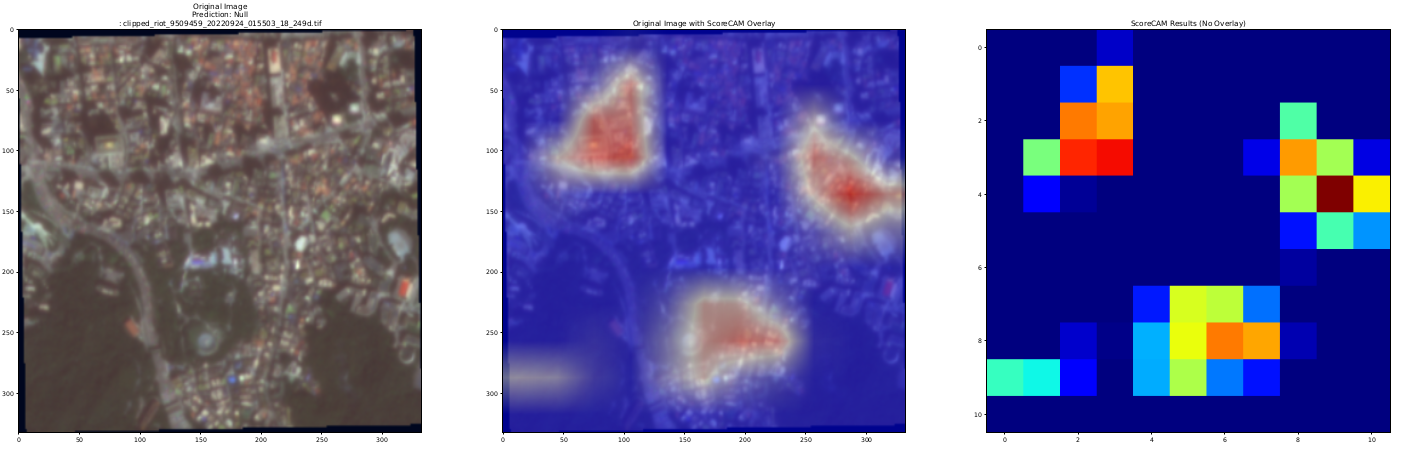
\includegraphics[width=0.75\linewidth]{noncontiguous_results.png}
    \caption{Score-CAM results displayed on the right of this figure represent a multiple regions of interest, regardless of the threshold set for consideration into a region of interest.}
    \label{fig:noncontiguous_ScoreCAM}
\end{figure}

%Another distinct issue that can arise with non-contiguous regions of interest, is if there are conflicts between classification.  When looking at non-contiguous results, such as the results in figure \ref{fig:noncontiguous_ScoreCAM}, it is possible that the region on interest in the upper left indicates one classification (i.e., a riot occurred), while the region in the upper right indicates a different classification (i.e., no riot occurred).   

Integral to the previously challenges is the underlying decision in determining what threshold to establish for consideration as a region of interest.  Before constructing the regions of interest, we must determine how much of the Score-CAM results should be used to consider.  If we set the threshold ($\ \epsilon $ in equation \ref{sat-cam_equation}) too low, we will consider too much of image.  If we consider too much of the image, the task of determining what in the image is being identified can be overwhelmed with too much non-essential information.  If we set the threshold$\ \epsilon$ too high, we will not consider enough of the image.  This will eliminate too much of the image, making identification, in terms of human interpretation, very challenging.  If we refer back to the sports stadium example discussed in Chapter \ref{sec:chapter3}, if we eliminate too much of the stadium because of a high threshold, we might only see some of the stadium making identification more challenging.



%----------------------------------------------------------------------------------------
%	SECTION 3
%----------------------------------------------------------------------------------------

\section{Dissertation Paper 3: Identification of conflict within Satellite Imagery }


\subsection{Major Research Question}
\textit{Can deep learning techniques enable the localization of conflict across a full-sized satellite image?}

While the first paper of my dissertation examines \textit{if} we can predict the likelihood of conflict using paired cases of images, and paper two explores \textit{why} these predictions are made, this leaves the question of if these tools can be operationally useful open.  While an algorithm that can discriminate between pairs of conflict and no-conflict cases may be useful, in practice it is unlikely that practitioners will have such a database.  More practically, they are likely to have many satellite scenes that they would like to identify probable locations of riots or protests.  While a model designed to take in pairs of images can accommodate this task, it requires additional modeling and testing in that broader context.  This chapter will fill that gap.

\subsubsection{Data}
My third paper will continue to leverage information from Planet, focusing on full images from the satellite sensors rather than clipped regions.  We plan to use the same source of data as specified in section \ref{sec:ch4_paper1_data}, which consists of 18,631 full satellite scenes distributed around the world. These images were collected from October 2017 to September 2022 and selected to be at least 24 hours prior to a conflict event.  An example of a single image collected from a satellite can be seen in figure \ref{fig:athens_baseimage}. 
 We also maintain a record of the latitude and longitude, as well as the clipped image, of the known riot for each full satellite scene.

%Our primary source of data is going to be the images we have previously downloaded.  These are full size satellite scenes of cities 24-48 hours prior to a known protest or riot.  Additionally we will use the pretrained ResNet18 from Chapter 3.   This network is trained to predict if a clipped 1-km box is from a riot or not from a riot.  

\subsubsection{Methods}
We will use our trained ResNet18 from chapter \ref{sec:chapter3} to identify the likely locations of riots and protests in full satellite scenes.  To accomplish this, we will take the following steps:
\begin{enumerate}
\item Create a grid that subsets the full satellite scene.
\item Systematically evaluate 1 $\ km^{2}$ boxes, encompassing the full satellite scene.
\item Collect results from step 2, to identify locations of probable riot or protest.
\end{enumerate}
In the first step of our methodology, we establish a grid that subsets the entire satellite scene into half kilometer boxes (see figure \ref{fig:grid_paper3}).  We subset the satellite scene, because we aim to evaluate the scene in a similar manner to a convolutional filter passing over a full image.  Our goal is to evaluate groups of subset half kilometer boxes in the same way a 2x2 convolutional filter captures the spatial relationship of four adjacent pixels in an input image, resulting in a single output value for the adjacent pixels.  We will evaluate four of the subset grids as a single clipped image and generate a single output, in our scenario a classification of riot or non-riot.  By subseting the full satellite scene into half kilometer boxes, we preserve the capability of our trained ResNet18 to evaluate each 2x2 grouping as an individual clipped image, similar to our data set in chapter \ref{sec:chapter3}.  This subseting of full satellite scenes will be unique to each individual scene.  As discussed in chapter \ref{sec:chapter3}, and highlighted in table \ref{tab:doves}, the spatial dimensions of images vary with each generation of satellite as well as the off-nadir angle from when the the image is captured.

\begin{figure}
    \centering
    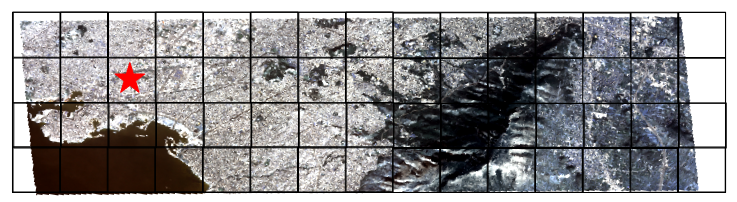
\includegraphics[width=0.75\linewidth]{Figures/grided_satimage.png}
    \caption{Example of grid that subsets entire satellite scene.  This image is not to scale, but represents a potential half kilometer grid that encompasses the full satellite scene.  In this example, there is a known feature(s) that causes a riot classification represented by a red star.  Imagery \textcopyright Planet Labs PBC 2023. All rights reserved.}
    \label{fig:grid_paper3}
\end{figure}

In the second step of our methodology, we evaluate the 2x2 adjacent half kilometer boxes across the full satellite scene.  Again, we build off the analogy of a convolutional filter sliding across an input image.  We will pad our satellite scene to account for data at the edge of the scene.  We implement a stride of one, to evaluate each half kilometer box multiple times.  An illustration of this process is shown in figure \ref{fig:eval_paper3}.  The purpose of subsetting the image and evaluating each half kilometer box as part of a 2x2 grouping, is to account for the unknown proximity relationship among spatial features that are important to riot classification.  This technique allows us to evaluate spatial features across a wider area of consideration, as opposed to limiting the spatial features to evaluation in the isolation of a single kilometer or half kilometer box. 

\begin{figure}
    \centering
    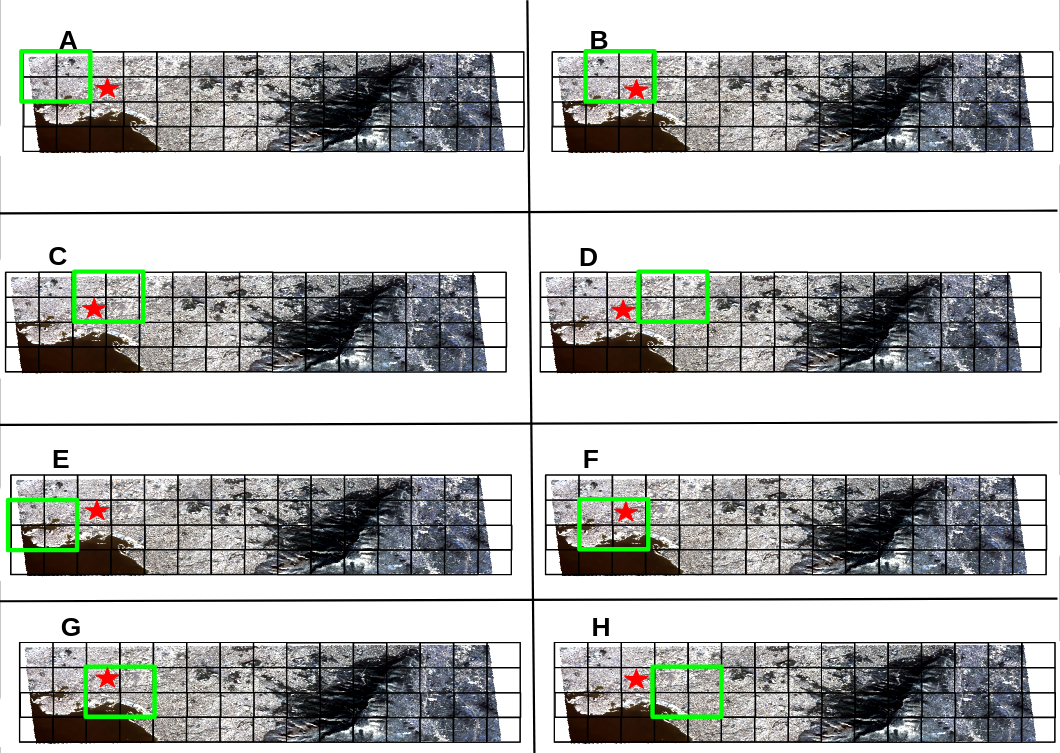
\includegraphics[width=1\linewidth]{Figures/eval_frames.png}
    \caption{This illustration is not to scale.  The green box represents the 2x2 convolutional filter used to evaluate the satellite scene.  Again, there is a known feature(s) that causes a riot classification represented by a red star.  The green box slides across the full scene.  In frames B, C, F, and G, all four of the half kilometer boxes would be marked as a riot.  In frames A, D, E, and H, none of the half kilometer boxes would be marked as a riot.  Imagery \textcopyright Planet Labs PBC 2023. All rights reserved.}
    \label{fig:eval_paper3}
\end{figure}

The third step is to collect the results of the second step to identify the probable locations for protests or riots.  Continuing with the 2x2 convolutional filter analogy, when the ResNet18 evaluates the four adjacent half kilometer boxes, all four are categorized as a riot or non-riot.  Each individual half kilometer box is evaluated four times, with different combinations of the surrounding boxes.  If the spatial features important to riot classification are present in a particular box, then that half kilometer box should be categorized as a riot four times.  While adjacent half kilometer boxes are categorized as a riot less than four times.  This will create a heat map across the full satellite scene, highlighting the particular regions in the image that are probable locations for riot or protest (see figure \ref{fig:heatmap_paper3}).  We then compare the heat map indicated locations to the known riot location to determine if the ResNet is able to determine the location of the riot or protest from a full satellite scene.

\begin{figure}
    \centering
    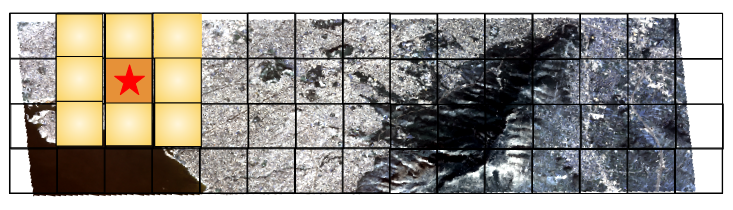
\includegraphics[width=0.75\linewidth]{Figures/heatmap_localized.png}
    \caption{The resulting heat map created during evaluation, that contains the spatial features that cause riot classification indicated by the red star.  Since the half kilometer box containing the red star was counted as a riot more often than its neighbors, this region appears as a hot spot that indicated probable riot or protest.  Illustration is not to scale.  Imagery \textcopyright Planet Labs PBC 2023. All rights reserved.}
    \label{fig:heatmap_paper3}
\end{figure}
There are two ways to validate our findings in step three.  The first is to measure the distance from the center of the region indicated in the heat map, to the latitude and longitude of the known riot.  The second is to compare how much the clipped image overlaps with the hot spots from the heat map.  It is currently unknown if our outlined methodology will result in the identification of a single riot or multiple riots.  We also do not know the size of any of the hot spots our methodology will create.  We are currently exploring the most appropriate manner for evaluation of performance in terms of accuracy, precision, recall, or other relevant measures.

There is potential to include further analysis related to explainability highlighted in section \ref{sec:paper_two}.  After identifying regions in the full image that are likely to have a protest, we can implement SAT-CAM to gain insight into the features driving classification.  It is currently unknown how the relationship between spatial features and their distribution impact classification.  Additionally, we do not know how spatial separation among important features influences classification across wider areas, such as full satellite scenes.  For example, large parks and the presence of government buildings might drive riot classification in a single one kilometer clipped image, but those same features when separated by a greater distance might no longer indicate a riot.


\subsection{Possible Challenges/Barriers}
There are a few potential challenges with this methodology.  One of the key assumptions in our training data is that there is only one riot or protest in each satellite scene, or at least there are no riots outside the ten kilometer exclusion area when the null clips were created (as described in chapter \ref{sec:chapter3}).  If there are other riots in the satellite scene, the trained network might correctly identify riot locations outside the known clip location, and based on our training data we would consider that a miss-classification.  

Another potential challenge identified for this study involves the methodology of analyzing entire satellite scenes to detect instances of riots or protests using a network originally trained on one-square-kilometer segments. The underlying assumption of our model posits that the spatial characteristics relevant to the classification task are less than one kilometer in size and that any spatial correlations critical for accurate classification occur within this distance. However, this assumption may not hold in all cases, as it is conceivable that certain spatial features or indicators of a riot or protest exceed this size limit or are dispersed beyond a kilometer, leading to potential inaccuracies in classification. This challenge underscores the need for a robust evaluation of the model's assumptions and its capability to generalize across varying spatial dimensions.

A further potential challenge originates from parameter choice in our methodology.  We opt for a half kilometer segmentation in order to evaluate each half kilometer box multiple times with its adjacent neighbors.  While this allows each segment to be classified multiple times, we might not be isolating the relevant spatial features enough.  We could attempt to compensate for this by decreasing the size of our grid.  For example we could use a quarter kilometer grid, and include a filter with a 4 x 4 block to construct a kilometer box for evaluation.  This would allow us to evaluate the relevant spatial feature more often, but it would also increase the computational cost.  We do not know the size of the features that are relevant to prediction, nor do we know if they are consistent in size.  So we are presented with an unknown constraint to the appropriate size of the grid to best capture the relevant features.  This problem is similar to the issue of required spatial resolution for object based image analysis \citep{blaschke2010object}






